\documentclass{cumcm}
\begin{document}
\begin{minipage}{0.9\textwidth}
\centering\LARGE\textbf{“同心协力”策略研究}

\end{minipage}
\begin{abstract}
本题在于考察分析同心球项目在不同情境下,通过调整团队队员发力的时机及力度,找出团队协作的最佳策略,使排球在鼓面上能持续颠起。\par
\begin{itemize}
\item \textbf{针对问题一分析}\quad 首先对于人数的一般值进行分析,确定绳长及人相对同心鼓的最佳站位和分布。我们将一次完整的颠球过程(鼓从初始位置出发到回到初始位置的过程)分为三个阶段,建立竖直平面内的运动模型.以排球和同心鼓的理想运动过程是稳定周期运动为切入点,对于周期内各个阶段的位移、时间关系设列运动关系方程。然后根据对同心鼓建立空间受力分析模型,使用得到的牛顿第二定律方程与前面的运动关系方程联立,得到各物理量值。计算出在最佳策略下,每位队员只需施加的大小为$6.25861N$的力,使鼓与排球碰撞,在碰撞结束$0.090s$后,施加$0.337s$的大小为$7.14003N$的力,使鼓回到原位置,完成一次周期。
\\
\item \textbf{问题二分析}\quad 该问题是一个旋转运动问题。首先需要对鼓和绳子进行几何分析,找出每个固定点的倾斜角度与鼓的倾斜角度,以及固定点的倾斜角度与此处牵拉绳子的旋转角度之间的关系。由于鼓是一个旋转対称体,所以可将八个固定点分成四组,每两个对称固定点为一组,建立力矩与转动惯量模型。分析序号$1$到序号$9$的施力力度及时机,找出每种情况对应的旋转主轴。再利用MATLAB编程,改变不同的参数,求出不同时刻鼓的倾斜角度。\\
\item \textbf{问题三分析}\quad\\
\item \textbf{问题四分析}\quad\\
\end{itemize}
\textbf{关键词} \quad 运动方程 \quad  MATLAB\quad 同心球 \quad 
\end{abstract}

\newpage
\section{问题重述}
\subsection{问题背景}
“同心协力”是一项需要团队高度协作的项目,不仅考察队员之间的默契程度,还锻炼了队员在压力环境中的心理承受能力,近年来受到了人们的热烈追捧。该项目的道具是一面在鼓身沿圆周均匀固定了多根绳子的牛皮双面鼓,以及一个富有弹性、气密性好的专用排球。项目开始时,团队成员每人牵拉一根绳子的末端,使鼓面保持水平,然后将球从鼓面正中心放下,队员找准时机同时用力将球颠起,使其能在鼓面上持续跳动而不落地,最终颠球次数最多的队伍获胜。
\subsection{问题的提出(题目重述)}
项目的目标是使球连续颠起次数尽可能多。现给定相关参数,包括所用双面鼓及排球的质量,鼓面直径,鼓身高度。同时要求团队队员人数不少于$8$人,各队员之间最小距离不小于$60cm$。排球最开始从鼓面中心正上方$40cm$处竖直下落,之后被颠起高度离鼓面距离应不小于$40cm$,否则项目终止。试通过数学建模,给出最佳策略。
\begin{enumerate}[(1)]
\item 假设每个队员都可以精确控制用力方向、时机和力度,讨论在此理想状态下团队的最佳协作策略,并给出该策略下的颠球高度。
\item 现实情况下,由于各队员之间用力不同,鼓面会出现一定程度的倾斜。试通过给定的参考数据,建立模型考察队员的发力时机和力度与某一特定时刻的鼓面倾斜角度关系。
\item 根据问题$2$中考虑了现实情况的模型,对问题$1$的策略做出适当调整。
\item 实际中,当鼓面发生倾斜时,球的跳动方向也不再竖直。现给定相关数据,计算出在可精确控制条件下所有队员的发力时机及力度,使球调整为竖直状态弹跳,并分析在现实情况中这种调整策略的实施效果。
\end{enumerate}

\section{模型假设}
\begin{enumerate}
\item 假设每根绳子均为柔性绳,每根绳子长度相同。
\item 不考虑风力以及空气阻力对排球运动的影响。
\item 当地重力加速度为$9.8kg/m^2$。
\item 排球是一个直径为$204mm$的五号标准排球。
\item 将排球视为一个均匀球壳。
\item 每位队员所隔距离相同,且手离地面高度相同(假定为$1.2m$),即各力作用位置沿鼓均匀分布。
\end{enumerate}

\newpage
\section{符号说明}
表\ref{table-symbol}列出了本文需要的符号。
\begin{table}[H]
  \centering
  \caption{符号说明}\label{table-symbol}
  \begin{tabular*}{\textwidth}{c|c|c|c}
  \hline
  符号 & 符号描述 & 符号 & 符号描述\\
  \hline
  $m_0$ & 鼓的质量 & $h$ & 鼓距离地面高度\\\
  $m_1$ & 排球质量 & $F_{i1}$ & 鼓加速上升时第$i$位队员施加力的大小($i$=1,2,3,\dots,$n$)\\
  $l$ & 绳子长度& $F_{i2}$ & 鼓减速下降时第$i$位队员施加力的大小($i$=1,2,3,\dots,$n$)\\
  $\varphi$ & 绳子与水平方向夹角 & $x_{10}$ & 球从最高处落下到碰撞时的高度差\\
  $v_{00}$ & 碰撞前鼓的速度 &  $x_{00}$ & 鼓从平衡位置到碰撞时的高度差\\
  $v_{01}$ & 碰撞后鼓的速度 &  $x_{01}$ & 鼓自由落体的高度差\\
  $v_{10}$ & 碰撞前球的速度 & $x_{02}$ & 鼓减速回到平衡位置的高度差\\
  $v_{11}$ & 碰撞后球的速度 & $v_{02}$ & 鼓自由落体结束时的高度差\\
  $a_1$ & 鼓加速上升时的加速度 & $a_2$ & 鼓减速下降时的加速度\\
  $r$ & 鼓面半径 & $\alpha$ & 鼓倾斜角度\\
  \hline
  \end{tabular*}
\end{table}


\section{问题分析}
\subsection{问题1分析}
题一是一个运动过程分析问题。因为我们考虑绳子为柔性绳,则施加力的方向沿绳方向。在理想情况下,我们可认为每位队员同时施加大小相等的力,即在此题中,$F_{i1}=F_1$,$F_{i2}=F_2$。假设在初始条件下鼓处于平衡位置,记为$s_0$。我们将一次颠球过程分为三个阶段,步骤如下:
\begin{enumerate}
\item 在第一阶段每位队员施加竖直向上的力$F_1$使鼓向上运动,到达$s_1$与排球碰撞,此时鼓上升高度为$x_{00}$,球下降的高度为$x_{10}$。在碰撞前鼓有一个竖直向上的速度$v_{00}$,球有一个竖直向下的速度$v_{10}$。我们考虑两者碰撞过程在瞬间完成,碰撞后鼓速度记为$v_{01}$,球速度记为$v_{11}$,方向均为竖直向上。
\item 在第二阶段,碰撞后鼓做自由落体运动,运动方向为先上升后下降,到达$s_2$,此时鼓速度为$v_{02}$,与碰撞处的高度差为$x_{01}$,而排球继续上升。
\item 在第三阶段,队员施加$F_2$的力使鼓做减速运动从$s_2$回到平衡位置,同时排球到达最高处,该阶段结束时鼓与排球的速度都为$0$。
\end{enumerate}
运动分析图如图(\ref{fig-buoy})所示:
\begin{figure}[H]
\centering
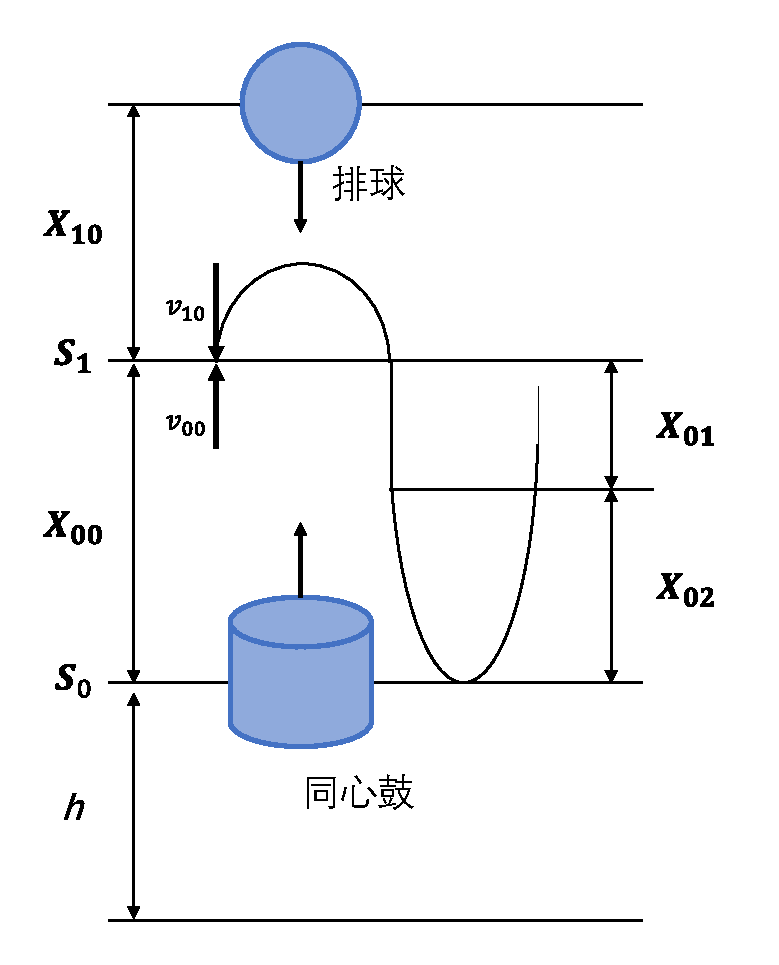
\includegraphics[width=0.8\textwidth]{img/question1.pdf}
\caption{问题一运动过程示意图(未考虑尺寸比例)}\label{fig-buoy}
\end{figure}

\subsection{问题2分析}
分析步骤如下:
\begin{enumerate}
\item 我们任意选取鼓面上两条半径$AD$,$AH$,长度为$r$,记它们之间夹角为$\gamma$,如图(\ref{figcircle})所示。
\begin{figure}[H]
  \begin{minipage}[t]{0.5\linewidth}   
    \centering   
    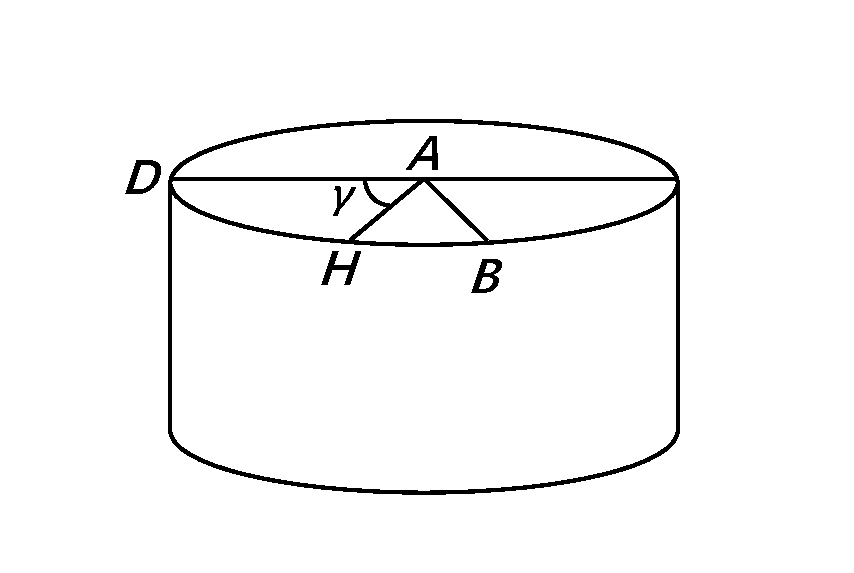
\includegraphics[width=0.8\textwidth]{img/circle.png}   
    \caption{鼓面倾斜示意图(一)}   
    \label{figcircle}   
  \end{minipage}   
   \begin{minipage}[t]{0.5\linewidth}   
      \centering   
      \includegraphics[width=0.8\textwidth]{img/change.png}   
      \caption{鼓面倾斜示意图(二)}   
      \label{fig:change}   
    \end{minipage} 
\end{figure}

\quad \quad
假设鼓面沿着与半径$AD$垂直方向的线$AB$倾斜,鼓平面从平面$ABCD$转到了平面$ABC_2D_2$(两平面均看成长方形),旋转角为$\alpha$,如图(\ref{fig:change})所示。$AC$为$AH$所在半径的延长线,则$AC$与$CB$之间夹角为$\gamma$,$AC_2$与$C_2B$之间夹角为$\gamma$。点$E$为点$C_2$在平面$ABCD$的投影,即$C_2E$垂直于$CB$,$AE$与$AB$夹角为$\eta$,角$\alpha_1$为$AC_2$与原平面所夹角。则有:\\
\begin{displaymath}
AC_2=\frac{C_2B}{sin\gamma}
\end{displaymath}
\begin{displaymath}
C_2E=C_2Bsin\alpha
\end{displaymath}
\begin{displaymath}
C_2E=AC_2sin\alpha_1
\end{displaymath}
由以上三式可得出$\alpha_1$与$\alpha$、$\gamma$之间关系为:
\begin{equation}
sin\alpha_1=sin\alpha cos\gamma
\end{equation}

\item 当鼓身上绳子的某一固定端与中心的连线倾斜了$\alpha$角时,我们该条绳角度倾斜了$\theta$角,如下图(\ref{fig:angel})所示。因为$\alpha$与$\theta$很小,所以我们近似可得:

\begin{displaymath}
l\theta=r\alpha
\end{displaymath}
不失一般性,我们可推广得到:
\begin{equation}
l\theta_i=r\alpha_i
\end{equation}
\begin{figure}[H]
\centering
\includegraphics[width=0.5\textwidth]{img/angel.png}
\caption{绳子改变角度示意图}\label{fig:angel}
\end{figure}

\item 由于鼓是一个旋转対称体,所以可将八个固定点分成四组,每两个对称固定点为一组。我们首先考察其中一个固定端。在鼓面为水平时,绳子与水平方向夹角为$\varphi$,当鼓面倾斜了$\alpha$角时,绳子与水平方向角度改变$\theta$,则该固定点处绳子与水平方向夹角变为$(\varphi-\theta)$,绳子所施加力$F_1$在平面$AC_2E$上点$H_2$的下方某处,我们可将力分解为竖直方向和沿$AC$方向的力。竖直方向力的大小为$F_1sin(\varphi-\theta_1)$,与直线$AB$距离为$rcos\gamma cos\alpha$;沿$AC$方向力的大小为$F_1cos(\varphi-\theta_1)$,再将其分解为与$AB$直线和与$AD$直线平行的两个力。$F_{AD}$大小为$F_1cos(\varphi-\theta_1)sin\eta$,与直线$AB$距离为$rsin\alpha_1$;因为$F_{AB}$与$AB$平行,所以在鼓倾斜时对力矩不会产生影响;而关于该固定点关于圆心中心对称处的固定端处绳子与竖直方向夹角变为$(\varphi+\theta)$,设该处力的大小为$F_2$,所能产生影响的两分解力大小分别为$F_2sin(\varphi-\theta_1)$,$F_2cos(\varphi-\theta_1)sin\eta$,与直线$AB$距离分别为$rcos\gamma cos\alpha$,$rsin\alpha_1$,建立出转动方程。 结合每组的转动方程,可得到关于鼓的转动模型。
\begin{figure}[H]
\centering
\includegraphics[width=0.8\textwidth]{img/fight.png}
\caption{双面鼓受力示意图}\label{fig:fight}
\end{figure}
\item 分析题目给定数据,选取旋转主轴:某一时刻的旋转主轴方向,即为与此时刻合力方向相垂直的鼓面直径所在方向。如图 (\ref{figmain})所示。在某时刻鼓上受到八个力的作用,根据牛顿第一定律,我们可对这八个力进行抵消,$F_1$和$F_2$为抵消后残余的力,$F$为两残余力的合力,它在平面$P$内,则此时的旋转主轴方向就为与平面$P$垂直的$ab$直径所在方向。利用MATLAB建立模型。

\begin{figure}[H]
\centering
\includegraphics[width=0.8\textwidth]{img/main.png}
\caption{旋转主轴示意图}\label{figmain}
\end{figure}

\item 对序号$1$到序号$9$给定的序号进行分析,我们发现$9$种情况可分为两种类型:对于序号$1$到序号$7$,以及序号$9$,旋转主轴只有一个,旋转主轴可由上述方法得到。而序号$8$在$-0.1s$和$0s$分别有两条不同的旋转主轴。我们首先通过MATLAB对另外八题的鼓面倾角求解,发现在同一时刻由于几位队员多施加了$10N$的力而引起的鼓面倾角变化,相对于队员由于施力时机提早了$0.1$而引起的鼓面倾角变化来说,可以忽略不计,所以我们仍可认为序号$8$的旋转主轴方向为$-0.1s$的旋转主轴方向。
\end{enumerate}

\subsection{问题3分析}

\subsection{问题4分析}
结合问题$(1)$、$(2)$、$(3)$三题的分析解答过程,综合对问题四进行分析。为简化问题,我们假设两次碰撞位置都在同一水平面上。
\begin{enumerate}
\item 我们首先进行运动过程分析。因为鼓对排球的作用力始终是垂直鼓面向上的,所以当排球反弹时相对竖直方向产生$1^{\circ}$时,说明鼓与排球碰撞时的运动方向夹$0.5^{\circ}$角,则鼓相对水平面的倾斜角度为$0.5^{\circ}$,我们记此时倾角为$-0.5^{\circ}$。所以若想要在下一次碰撞时将排球调整为竖直状态弹跳,则应该使排球朝对称方向倾斜$0.5^{\circ}$。如图(\ref{fig:exercise})所示。
\begin{figure}[H]
\centering
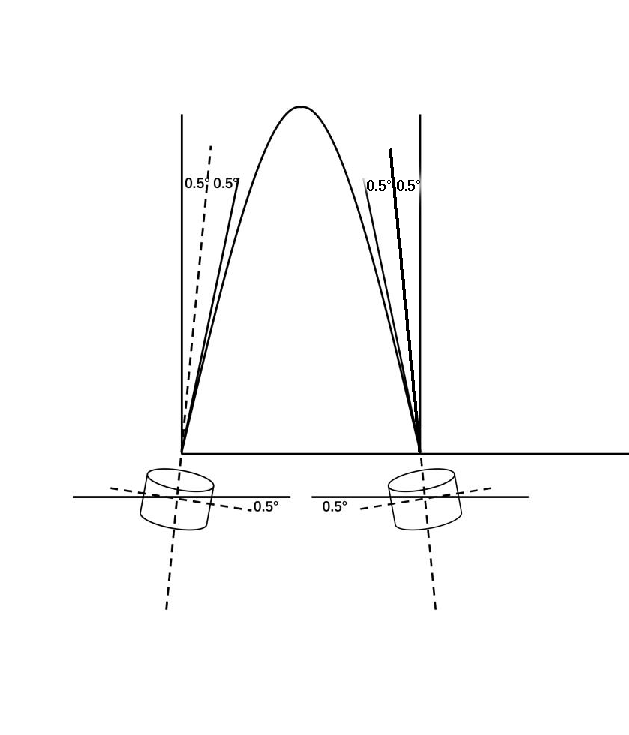
\includegraphics[width=0.8\textwidth]{img/exercise.pdf}
\caption{旋转主轴示意图}\label{fig:exercise}
\end{figure}
\item 假设此题中鼓收到的合力为$800N$。对排球在空中的运动进行分析,可计算得到两次碰撞的间隔时间。通过问题一的分析,我们知道在此次碰撞后到下一次碰撞前,鼓经历自由落体运动,减速下降,以及加速上升三个阶段。因为在此题中,我们无需考虑排球上升高度,所以为简化问题,可假定减速加速两过程所施加的力是一样的。同时由于碰撞时鼓的速度不可知,我们可假定碰撞后鼓以速度0自由落体。可计算得到队员作用力的时机、作用时间。
\item 在开始时,我们假设$10$位队员每人施加力的时机和力度都相同。保持原有的合力大小不变,逐渐增加一位队员施加力,减少其余队员施加力,利用MATLAB对该过程进行模拟分析。
\end{enumerate}


\subsection{问题1的解答}
\begin{enumerate}
\item \textbf{绳长计算}\\
我们假设团队队员共有$n$人,每人之间的距离为最小距离$60cm$。队员牵拉绳子的水平投影线的延长线交于绳子固定端所在圆的圆心$A$,则该圆心与两队员队员所站位置可构成水平的等腰三角形,三角形顶角为$\frac{360^{\circ}}{n}$,三角形底角角度为($90^{\circ}-\frac{180^{\circ}}{n}$),如下图所示:
\begin{figure}[H]
\centering
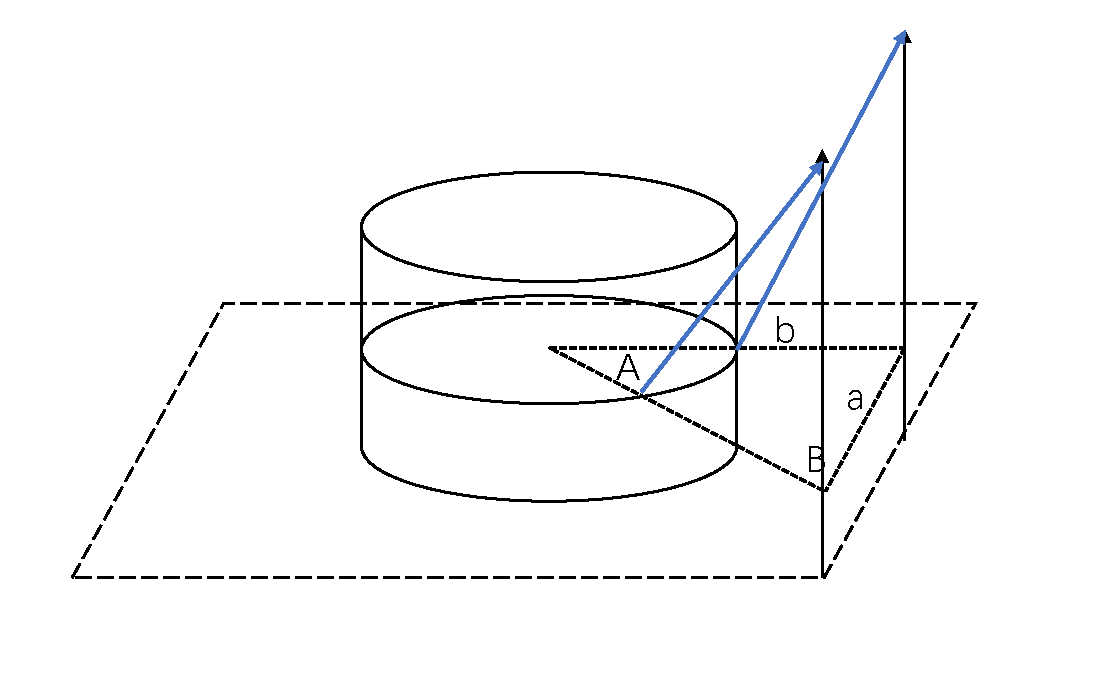
\includegraphics[width=0.8\textwidth]{img/string.pdf}
\caption{绳长计算示意图}
\end{figure}
由正弦定理可得:
\begin{displaymath}
\frac{a}{sinA}=\frac{b}{sinB}
\end{displaymath}
即:
\begin{displaymath}
\frac{60}{sin({\frac{360^{\circ}}{n}})}=\frac{b}{sin({90^{\circ}-\frac{180^{\circ}}{n}})}
\end{displaymath}
解得$b$的长度为:
\begin{displaymath}
b=\frac{30}{sin( \frac{180^{\circ}}{n})}
\end{displaymath}
又因为绳子与竖直方向夹角为$\varphi$,所以绳子长度可以表示为:
\begin{equation}
l=\frac{b-r}{cos\varphi}=\frac{\frac{30}{sin(\frac{180^{\circ}}{n})}-r}{cos\varphi}
\end{equation}
\item \textbf{运动计算}\\
在最佳协作策略下,每位队员都想要使自己施加的力尽可能小,持续时间尽可能短。这样我们可以假设排球所能到达的最高高度恰好为$40cm$。
在第一阶段中,排球从最高处自由落到碰撞位置的时间与鼓从$s_0$上升到碰撞位置的时间相等,可列公式:
\begin{equation}
\frac{v_{00}}{a_1}=\frac{v_{10}}{g}
\end{equation}
且有$x_{00}+x_{10}=0.4$,即:
\begin{equation}
\frac{v^2_{10}}{2g}+\frac{v^2_{00}}{2a_1}=0.4
\end{equation}
在二、三、阶段中,排球从碰撞位置回到最高点的时间与鼓从碰撞位置回到$s_0$的时间相等,可列公式:
\begin{equation}
\frac{v_{11}}{g}=\frac{v_{02}+v_{01}}{g}+\frac{v_{02}}{a_2}
\end{equation}
且有$x_{10}+x_{01}+x_{02}=0.4$,则:
\begin{equation}
\frac{v^2_{11}}{2g}+\frac{(v^2_{02}-v^2_{01})}{g}+\frac{v^2_{02}}{a_2}=0.4
\end{equation}
排球做自由落体运动,在同一高度时速度大小相同,则有:
\begin{equation}
v_{11}=v_{10}
\end{equation}
碰撞时,由动量守恒可列公式:
\begin{equation}
m_0v_{00}-m_1v_{11}=m_0v_{01}+m_1v_{11}
\end{equation}
通过查阅相关资料,我们设定碰撞恢复系数大小为$0.74$,所列公式为:
\begin{equation}
e=\frac{v_{11}-v_{01}}{v_{00}+v_{11}}
\end{equation}
我们假设参与人数为$8$人,在最佳策略下每人施加力应尽可能小,则绳子与竖直方向夹角应尽可能小。所以此时$h=0$,即$s_0$在水平地面上。手的作用高度与绳子在鼓身固定端的高度差为$1.2-(\frac{0.22}{2})=1.09m$。
\begin{equation}
sin\varphi=\frac{1.09}{l}
\end{equation}
\item \textbf{计算求解}\\
结合方程$(3)$到方程$(11)$,利用MATLAB求解,得到结果:
$$v_{00}=0.593537m/s$$
$$v_{01}=0.2157m/s$$
$$v_{02}=0.669324m/s$$
$$v_{11}=v_{10}=2.51891m/s$$
$$F_1=6.25861N$$ 
$$F_2=7.14003N$$
\quad \quad
算得第一阶段时间为$0.257s$,第二阶段时间为$0.090s$,第三阶段时间为$0.337s$。
所以最佳策略为当球从最高处下落时,每位队员施加$6.25861N$的力,持续时间为$0.257s$,与排球碰撞,使排球弹起,最高点仍能回到$40cm$,碰撞$0.090s$后,每位队员施加$7.14003N$大小的力,持续$0.337s$,使鼓减速回到$s_0$。

\end{enumerate}

\subsection{问题2的解答}
在问题二中,$sin\varphi$计算结果为$0.0647$。
\begin{figure}[H]
\centering
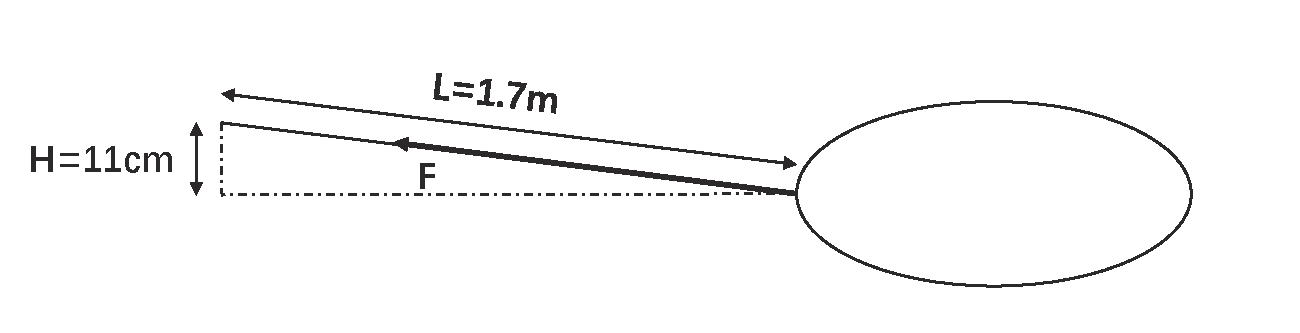
\includegraphics[width=0.8\textwidth]{img/string1.pdf}
\caption{绳长计算示意图}
\end{figure}
通过对问题二的分析,我们可将八个固定端分成四组,每两个相对称的固定端为一组,某一固定端转动方程为:
\begin{equation}
J\beta_{1i}= F_{1i}sin(\varphi-\theta_i)rcos\gamma cos\alpha- F_{1i}cos(\varphi-\theta_i)rsin\eta sin\varphi_i
\end{equation}
其对称处转动方程为:
\begin{equation}
J \beta_{2i}= F_{2i}sin(\varphi+\theta_i)rcos\gamma cos\alpha+F_{2i}cos(\varphi+\theta_i)rsin\eta sin\varphi_i
\end{equation}
综合所有固定端,得到鼓的转动方程如下:
\begin{equation}
J \beta=\sum_{i=1}^4 (J\beta_{i1}-J\beta_{i2})
\end{equation}
\quad \quad
结合公式$(1)$、$(2)$、$(12)$、$(13)$、$(14)$, 利用MATLAB进行小步长求解,得到结果如表\ref{table-sym}所示。
由于初始时,每位队员施加力的力度和时机不同,我们假定在开始时由于施力不均而造成鼓面旋转的方向为正方向。
\begin{table}[H]
\centering
\caption{鼓面倾斜角度结果}\label{table-sym}
\begin{tabular}{|c|c|c|c|c|c|c|c|c|c|c|}
\hline
序号 & 用力参数 & 1    & 2    & 3  & 4    & 5    & 6  & 7  & 8    & 鼓面倾角(度) \\
\hline
1  & 发力时机 & 0    & 0    & 0  & 0    & 0    & 0  & 0  & 0    &   $0.198926^{\circ}$ \\
   & 用力大小 & 90   & 80   & 80 & 80   & 80   & 80 & 80 & 80   &       \\
\hline
2  & 发力时机 & 0    & 0    & 0  & 0    & 0    & 0  & 0  & 0    &    $0.361033^{\circ}$ \\
   & 用力大小 & 90   & 90   & 80 & 80   & 80   & 80 & 80 & 80   &         \\
\hline
3  & 发力时机 & 0    & 0    & 0  & 0    & 0    & 0  & 0  & 0    &    $0.154996^{\circ}$ \\
   & 用力大小 & 90   & 80   & 80 & 90   & 80   & 80 & 80 & 80   &         \\
\hline
4  & 发力时机 & -0.1 & 0    & 0  & 0    & 0    & 0  & 0  & 0    &    $-2.33284^{\circ}$ \\
   & 用力大小 & 80   & 80   & 80 & 80   & 80   & 80 & 80 & 80   &         \\
\hline
5  & 发力时机 & -0.1 & -0.1 & 0  & 0    & 0    & 0  & 0  & 0    &    $-3.90435^{\circ}$ \\
   & 用力大小 & 80   & 80   & 80 & 80   & 80   & 80 & 80 & 80   &         \\
\hline
6  & 发力时机 & -0.1 & 0    & 0  & -0.1 & 0    & 0  & 0  & 0    &    $-1.9634^{\circ}$  \\
   & 用力大小 & 80   & 80   & 80 & 80   & 80   & 80 & 80 & 80   &         \\
\hline
7  & 发力时机 & -0.1 & 0    & 0  & 0    & 0    & 0  & 0  & 0    &    $-2.49741^{\circ}$ \\
   & 用力大小 & 90   & 80   & 80 & 80   & 80   & 80 & 80 & 80   &         \\
\hline
8  & 发力时机 & 0    & -0.1 & 0  & 0    & -0.1 & 0  & 0  & 0    &   $ -1.95983^{\circ}$ \\
   & 用力大小 & 90   & 80   & 80 & 90   & 80   & 80 & 80 & 80   &         \\
\hline
9  & 发力时机 & 0    & 0    & 0  & 0    & -0.1 & 0  & 0  & -0.1 &   $ -2.14966^{\circ}$ \\
   & 用力大小 & 90   & 80   & 80 & 90   & 80   & 80 & 80 & 80   &        \\
\hline
\end{tabular}
\end{table}
\subsection{问题3解答}


\subsection{问题4解答}
\begin{enumerate}
\item \textbf{排球运动分析}\\
排球在空中做加速度恒为$g=9.8m/s$的运动,且能达到的最高高度为$h=60cm$,所以根据运动方程:
\begin{displaymath}
\frac{1}{2}gt^2=h
\end{displaymath}
得到在空中运动时间为$2t=0.670s$,即两次碰撞间隔时间为$0.670s$。
\item\textbf{鼓运动计算}\\
我们假设鼓自由落体时间为$t_1$,变速运动时间为$t_2$,加速度为$a$,由于自由落体与变速运动两阶段位移相等。所以有:
\begin{equation}
\frac{1}{2}gt^2=-gt_1t_2+\frac{1}{2}at_2^2
\end{equation}
两次碰撞间隔,鼓运动时间与排球运动时间相等,可得等式:
\begin{equation}
t_1+t_2=2t
\end{equation}
我们仍假设鼓面初始位置较绳子水平时下降 11 cm鼓的加速度由公式代入数据得$sin\varphi$为0.055。
\begin{equation}
a=\frac{Fsin\varphi-mg}{m}=2.422m/s^2
\end{equation}
综合式子$(15)$到$(17)$,可计算得到$t_1$为$0.1804s$,$t_2$为$0.5193s$。
\item \textbf{排球受力分析}\\
在变速运动阶段,鼓由于受力不均而发生倾斜。因为我们想要使鼓的倾斜角度从$-0.5^{\circ}$变为$0.5^{\circ}$,所以当鼓水平时刚好为变速运动中间时刻。
\end{enumerate}
\section{模型总结}

\subsection{模型优点}

\subsection{模型缺点}


\bibliographystyle{plain}
\bibliography{ref}
\begin{thebibliography}{99}
\bibitem{1}
\bibitem{2}
\end{thebibliography}

\newpage
\appendix
\textbf{附录}
\section{问题一求解代码}
\begin{lstlisting}
clc
clear
syms n h step F1 F2 v00 v11 v01 v02 h11 n
% e 为鼓与球碰撞的恢复系数。
e = 0.74; m0 = 3.6; m1 = 0.27; g = 9.8; 
% h_min 为球颠起后需要距离鼓的最小距离40cm。
h_min = 0.4;
% step 为计算鼓上升时间的每次步长,单位为秒。
step = 0.001;
% l = input('Please input the length of the rope');
n = input('Please input the number of students:');
h = input('Please input the height of the hand:');
% n = 8; 
% h = 1.2;
% h0 为鼓距离地面的距离。
h0 = 0.11;
% alpha 人与人之间的角度。
alpha = 360/n;
% 绳长
lx = sqrt(0.6^2 / (2 * (1 - cos(alpha))));
ly = h - h0;
l = sqrt(lx^2 + ly^2);

cos_phi0 = ly / l;

a1 = (n * F1 * cos_phi0 - m0 * g)/m0;
a2 = (n * F2 * cos_phi0 - m0 * g)/m0;

equ1 = m0 * v00 - m1 * v11 == m0 * v01 + m1 * v11;
equ2 = (v11 - v01) / (v00 + v11) == e;
equ3 = a1 * v11 == g * v00;
equ4 = v11/g == (v02 + v01)/g + v02/a2;
equ5 = v11^2/g + v00^2/a1 == 0.8;
equ6 = v11^2/g + (v02^2 - v01^2)/g + v02^2/a2 == 0.8;
equ = [equ1, equ2, equ3, equ4, equ5, equ6];
[F1, F2, v00, v01, v02, v11] = solve(equ, [F1, F2, v00, v01, v02, v11]);
fprintf('施加的力F1为:%.5f\n施加的力F2为:%.5f\n',F1(2), F2(2));

% a2 = (n * F2(2) * cos_phi0 - m0 * g)/m0
% (v02(2)^2 - v01(2)^2)/(2*g) + v02(2)^2/(2*a2) + v11(2)^2/(2*g)
\end{lstlisting}

\section{问题二代码}
\begin{lstlisting}
\end{lstlisting}
\end{document}
